\documentclass[twoside]{book}

% Packages required by doxygen
\usepackage{calc}
\usepackage{doxygen}
\usepackage{graphicx}
\usepackage[utf8]{inputenc}
\usepackage{makeidx}
\usepackage{multicol}
\usepackage{multirow}
\usepackage{textcomp}
\usepackage[table]{xcolor}

% NLS support packages
Portuguese
% Font selection
\usepackage[T1]{fontenc}
\usepackage{mathptmx}
\usepackage[scaled=.90]{helvet}
\usepackage{courier}
\usepackage{amssymb}
\usepackage{sectsty}
\renewcommand{\familydefault}{\sfdefault}
\allsectionsfont{%
  \fontseries{bc}\selectfont%
  \color{darkgray}%
}
\renewcommand{\DoxyLabelFont}{%
  \fontseries{bc}\selectfont%
  \color{darkgray}%
}

% Page & text layout
\usepackage{geometry}
\geometry{%
  a4paper,%
  top=2.5cm,%
  bottom=2.5cm,%
  left=2.5cm,%
  right=2.5cm%
}
\tolerance=750
\hfuzz=15pt
\hbadness=750
\setlength{\emergencystretch}{15pt}
\setlength{\parindent}{0cm}
\setlength{\parskip}{0.2cm}
\makeatletter
\renewcommand{\paragraph}{%
  \@startsection{paragraph}{4}{0ex}{-1.0ex}{1.0ex}{%
    \normalfont\normalsize\bfseries\SS@parafont%
  }%
}
\renewcommand{\subparagraph}{%
  \@startsection{subparagraph}{5}{0ex}{-1.0ex}{1.0ex}{%
    \normalfont\normalsize\bfseries\SS@subparafont%
  }%
}
\makeatother

% Headers & footers
\usepackage{fancyhdr}
\pagestyle{fancyplain}
\fancyhead[LE]{\fancyplain{}{\bfseries\thepage}}
\fancyhead[CE]{\fancyplain{}{}}
\fancyhead[RE]{\fancyplain{}{\bfseries\leftmark}}
\fancyhead[LO]{\fancyplain{}{\bfseries\rightmark}}
\fancyhead[CO]{\fancyplain{}{}}
\fancyhead[RO]{\fancyplain{}{\bfseries\thepage}}
\fancyfoot[LE]{\fancyplain{}{}}
\fancyfoot[CE]{\fancyplain{}{}}
\fancyfoot[RE]{\fancyplain{}{\bfseries\scriptsize Gerado em Sexta, 25 de Agosto de 2017 10\-:54\-:40 para Trabalho 1 -\/ Software Básico por Doxygen }}
\fancyfoot[LO]{\fancyplain{}{\bfseries\scriptsize Gerado em Sexta, 25 de Agosto de 2017 10\-:54\-:40 para Trabalho 1 -\/ Software Básico por Doxygen }}
\fancyfoot[CO]{\fancyplain{}{}}
\fancyfoot[RO]{\fancyplain{}{}}
\renewcommand{\footrulewidth}{0.4pt}
\renewcommand{\chaptermark}[1]{%
  \markboth{#1}{}%
}
\renewcommand{\sectionmark}[1]{%
  \markright{\thesection\ #1}%
}

% Indices & bibliography
\usepackage{natbib}
\usepackage[titles]{tocloft}
\setcounter{tocdepth}{3}
\setcounter{secnumdepth}{5}
\makeindex

% Hyperlinks (required, but should be loaded last)
\usepackage{ifpdf}
\ifpdf
  \usepackage[pdftex,pagebackref=true]{hyperref}
\else
  \usepackage[ps2pdf,pagebackref=true]{hyperref}
\fi
\hypersetup{%
  colorlinks=true,%
  linkcolor=blue,%
  citecolor=blue,%
  unicode%
}

% Custom commands
\newcommand{\clearemptydoublepage}{%
  \newpage{\pagestyle{empty}\cleardoublepage}%
}


%===== C O N T E N T S =====

\begin{document}

% Titlepage & ToC
\hypersetup{pageanchor=false}
\pagenumbering{roman}
\begin{titlepage}
\vspace*{7cm}
\begin{center}%
{\Large Trabalho 1 -\/ Software Básico }\\
\vspace*{1cm}
{\large Gerado por Doxygen 1.8.6}\\
\vspace*{0.5cm}
{\small Sexta, 25 de Agosto de 2017 10:54:40}\\
\end{center}
\end{titlepage}
\clearemptydoublepage
\tableofcontents
\clearemptydoublepage
\pagenumbering{arabic}
\hypersetup{pageanchor=true}

%--- Begin generated contents ---
\chapter{Índice dos ficheiros}
\section{Lista de ficheiros}
Lista de todos os ficheiros com uma breve descrição\-:\begin{DoxyCompactList}
\item\contentsline{section}{\hyperlink{assembler_8cpp}{assembler.\-cpp} }{\pageref{assembler_8cpp}}{}
\item\contentsline{section}{\hyperlink{assembler_8h}{assembler.\-h} }{\pageref{assembler_8h}}{}
\item\contentsline{section}{\hyperlink{languagedefinition_8h}{languagedefinition.\-h} }{\pageref{languagedefinition_8h}}{}
\item\contentsline{section}{\hyperlink{lexer_8cpp}{lexer.\-cpp} }{\pageref{lexer_8cpp}}{}
\item\contentsline{section}{\hyperlink{lexer_8h}{lexer.\-h} }{\pageref{lexer_8h}}{}
\item\contentsline{section}{\hyperlink{main_8cpp}{main.\-cpp} }{\pageref{main_8cpp}}{}
\item\contentsline{section}{\hyperlink{msgs__pt_8h}{msgs\-\_\-pt.\-h} }{\pageref{msgs__pt_8h}}{}
\item\contentsline{section}{\hyperlink{preprocessor_8cpp}{preprocessor.\-cpp} }{\pageref{preprocessor_8cpp}}{}
\item\contentsline{section}{\hyperlink{preprocessor_8h}{preprocessor.\-h} }{\pageref{preprocessor_8h}}{}
\end{DoxyCompactList}

\chapter{Documentação do ficheiro}
\hypertarget{main_8cpp}{\section{Referência ao ficheiro main.\-cpp}
\label{main_8cpp}\index{main.\-cpp@{main.\-cpp}}
}
{\ttfamily \#include $<$stdio.\-h$>$}\\*
{\ttfamily \#include $<$stdlib.\-h$>$}\\*
{\ttfamily \#include $<$ctype.\-h$>$}\\*
{\ttfamily \#include $<$string.\-h$>$}\\*
{\ttfamily \#include $<$unistd.\-h$>$}\\*
{\ttfamily \#include \char`\"{}mensagens.\-h\char`\"{}}\\*
{\ttfamily \#include \char`\"{}preprocessador.\-h\char`\"{}}\\*
{\ttfamily \#include \char`\"{}montador.\-h\char`\"{}}\\*
Diagrama de dependências de inclusão para main.\-cpp\-:
\nopagebreak
\begin{figure}[H]
\begin{center}
\leavevmode
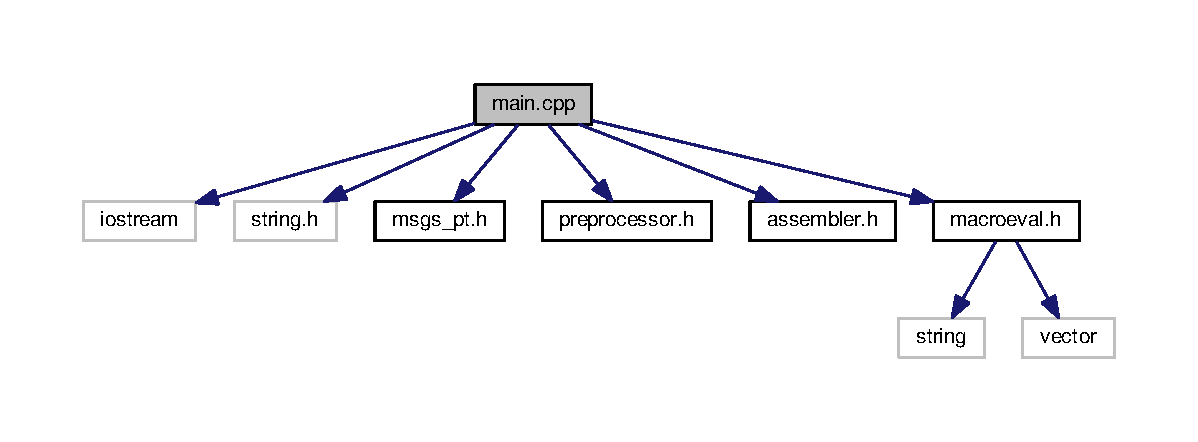
\includegraphics[width=350pt]{main_8cpp__incl}
\end{center}
\end{figure}
\subsection*{Funções}
\begin{DoxyCompactItemize}
\item 
int \hyperlink{main_8cpp_a3c04138a5bfe5d72780bb7e82a18e627}{main} (int argc, char $\ast$$\ast$argv)
\end{DoxyCompactItemize}


\subsection{Documentação das funções}
\hypertarget{main_8cpp_a3c04138a5bfe5d72780bb7e82a18e627}{\index{main.\-cpp@{main.\-cpp}!main@{main}}
\index{main@{main}!main.cpp@{main.\-cpp}}
\subsubsection[{main}]{\setlength{\rightskip}{0pt plus 5cm}int main (
\begin{DoxyParamCaption}
\item[{int}]{argc, }
\item[{char $\ast$$\ast$}]{argv}
\end{DoxyParamCaption}
)}}\label{main_8cpp_a3c04138a5bfe5d72780bb7e82a18e627}
Trabalho 1 -\/ Software Básico

\begin{DoxyAuthor}{Autores}
Rafael Lima e João Pedro Franch 
\end{DoxyAuthor}
\begin{DoxyVersion}{Versão}
0.\-2 
\end{DoxyVersion}
Pré Processamento (E\-Q\-U, I\-F) 

Definido na linha 18 do ficheiro main.\-cpp.



Grafo de chamadas desta função\-:
\nopagebreak
\begin{figure}[H]
\begin{center}
\leavevmode
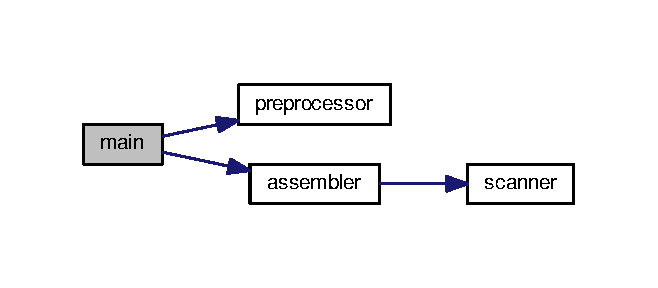
\includegraphics[width=240pt]{main_8cpp_a3c04138a5bfe5d72780bb7e82a18e627_cgraph}
\end{center}
\end{figure}



\hypertarget{mensagens_8h}{\section{Referência ao ficheiro mensagens.\-h}
\label{mensagens_8h}\index{mensagens.\-h@{mensagens.\-h}}
}


Mensagens do programa.  


Este grafo mostra quais são os ficheiros que incluem directamente ou indirectamente este ficheiro\-:
\nopagebreak
\begin{figure}[H]
\begin{center}
\leavevmode
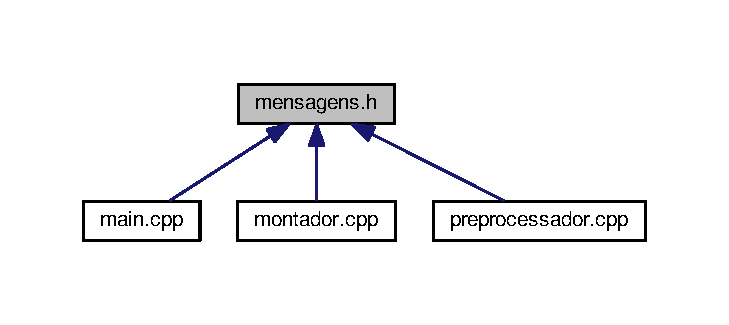
\includegraphics[width=350pt]{mensagens_8h__dep__incl}
\end{center}
\end{figure}
\subsection*{Macros}
\begin{DoxyCompactItemize}
\item 
\#define \hyperlink{mensagens_8h_ab7b84c63c73a6cb6e2fdd3fe99a98fd2}{M\-S\-G\-\_\-\-E\-R\-R\-O\-\_\-\-A\-R\-G\-U\-M\-E\-N\-T\-O\-S}~\char`\"{}\textbackslash{}t\-Numero de argumentos invalido\textbackslash{}n\textbackslash{}t\-Sao necessarios 3 argumentos\-: o nome do arquivo a ser compilado, a opcao e o nome do arquivo objeto\textbackslash{}n\char`\"{}
\item 
\#define \hyperlink{mensagens_8h_ac7982637c7546825516702569d22a7be}{M\-S\-G\-\_\-\-E\-R\-R\-O\-\_\-\-S\-E\-G\-U\-N\-D\-O\-\_\-\-A\-R\-G\-U\-M\-E\-N\-T\-O}~\char`\"{}\textbackslash{}t\-O segundo argumento esta mal formado\-:\textbackslash{}n\textbackslash{}t -\/p\-: pre-\/processado\textbackslash{}n\textbackslash{}t -\/m\-: arquivo apos a resolucao das macros\textbackslash{}n\textbackslash{}t -\/o\-: para o arquivo objeto final\textbackslash{}n\char`\"{}
\item 
\#define \hyperlink{mensagens_8h_ab6fed1316f07e7ac4df8ebc4527cc1a0}{M\-S\-G\-\_\-\-E\-R\-R\-O}~\char`\"{}\textbackslash{}t\-Erro 9000\textbackslash{}n\char`\"{}
\item 
\#define \hyperlink{mensagens_8h_a267d6b3302ee9d622830c98eaa83f5d2}{M\-S\-G\-\_\-\-E\-R\-R\-O\-\_\-\-A\-R\-Q\-U\-I\-V\-O}~\char`\"{}\textbackslash{}t\-Problemas ao abrir arquivo\textbackslash{}n\char`\"{}
\item 
\#define \hyperlink{mensagens_8h_afc8c62691ddfa0aab97a4602b5fb30dc}{M\-S\-G\-\_\-\-E\-R\-R\-O\-\_\-\-I\-N\-S\-T\-R\-U\-C\-A\-O\-\_\-\-I\-N\-V\-A\-L\-I\-D\-A}~\char`\"{}\textbackslash{}t Instrução Inválida\textbackslash{}n\char`\"{}
\item 
\#define \hyperlink{mensagens_8h_a5858905dc8fe4e7d4b1e425bdf3a63e5}{P\-R\-I\-N\-T\-\_\-\-E\-R\-R\-O}(arquivo, linha\-Code, M\-S\-G)
\item 
\#define \hyperlink{mensagens_8h_ab9c5e6683113b397e37e981ef6c34613}{P\-R\-I\-N\-T\-\_\-\-E\-R\-R\-O\-\_\-\-I\-N\-S\-T\-R\-U\-C\-A\-O}(linha\-Code, I\-N\-S\-T)~cout $<$$<$ \char`\"{}Linha \char`\"{} $<$$<$ linha\-Code +1 $<$$<$ \char`\"{} \-: \char`\"{}$<$$<$ string(I\-N\-S\-T) $<$$<$\char`\"{} -\/$>$ Instrução Inválida\textbackslash{}n\char`\"{}
\end{DoxyCompactItemize}


\subsection{Descrição detalhada}
Mensagens do programa. 

Definido no ficheiro \hyperlink{mensagens_8h_source}{mensagens.\-h}.



\subsection{Documentação das macros}
\hypertarget{mensagens_8h_ab6fed1316f07e7ac4df8ebc4527cc1a0}{\index{mensagens.\-h@{mensagens.\-h}!M\-S\-G\-\_\-\-E\-R\-R\-O@{M\-S\-G\-\_\-\-E\-R\-R\-O}}
\index{M\-S\-G\-\_\-\-E\-R\-R\-O@{M\-S\-G\-\_\-\-E\-R\-R\-O}!mensagens.h@{mensagens.\-h}}
\subsubsection[{M\-S\-G\-\_\-\-E\-R\-R\-O}]{\setlength{\rightskip}{0pt plus 5cm}\#define M\-S\-G\-\_\-\-E\-R\-R\-O~\char`\"{}\textbackslash{}t\-Erro 9000\textbackslash{}n\char`\"{}}}\label{mensagens_8h_ab6fed1316f07e7ac4df8ebc4527cc1a0}


Definido na linha 11 do ficheiro mensagens.\-h.

\hypertarget{mensagens_8h_ab7b84c63c73a6cb6e2fdd3fe99a98fd2}{\index{mensagens.\-h@{mensagens.\-h}!M\-S\-G\-\_\-\-E\-R\-R\-O\-\_\-\-A\-R\-G\-U\-M\-E\-N\-T\-O\-S@{M\-S\-G\-\_\-\-E\-R\-R\-O\-\_\-\-A\-R\-G\-U\-M\-E\-N\-T\-O\-S}}
\index{M\-S\-G\-\_\-\-E\-R\-R\-O\-\_\-\-A\-R\-G\-U\-M\-E\-N\-T\-O\-S@{M\-S\-G\-\_\-\-E\-R\-R\-O\-\_\-\-A\-R\-G\-U\-M\-E\-N\-T\-O\-S}!mensagens.h@{mensagens.\-h}}
\subsubsection[{M\-S\-G\-\_\-\-E\-R\-R\-O\-\_\-\-A\-R\-G\-U\-M\-E\-N\-T\-O\-S}]{\setlength{\rightskip}{0pt plus 5cm}\#define M\-S\-G\-\_\-\-E\-R\-R\-O\-\_\-\-A\-R\-G\-U\-M\-E\-N\-T\-O\-S~\char`\"{}\textbackslash{}t\-Numero de argumentos invalido\textbackslash{}n\textbackslash{}t\-Sao necessarios 3 argumentos\-: o nome do arquivo a ser compilado, a opcao e o nome do arquivo objeto\textbackslash{}n\char`\"{}}}\label{mensagens_8h_ab7b84c63c73a6cb6e2fdd3fe99a98fd2}


Definido na linha 9 do ficheiro mensagens.\-h.

\hypertarget{mensagens_8h_a267d6b3302ee9d622830c98eaa83f5d2}{\index{mensagens.\-h@{mensagens.\-h}!M\-S\-G\-\_\-\-E\-R\-R\-O\-\_\-\-A\-R\-Q\-U\-I\-V\-O@{M\-S\-G\-\_\-\-E\-R\-R\-O\-\_\-\-A\-R\-Q\-U\-I\-V\-O}}
\index{M\-S\-G\-\_\-\-E\-R\-R\-O\-\_\-\-A\-R\-Q\-U\-I\-V\-O@{M\-S\-G\-\_\-\-E\-R\-R\-O\-\_\-\-A\-R\-Q\-U\-I\-V\-O}!mensagens.h@{mensagens.\-h}}
\subsubsection[{M\-S\-G\-\_\-\-E\-R\-R\-O\-\_\-\-A\-R\-Q\-U\-I\-V\-O}]{\setlength{\rightskip}{0pt plus 5cm}\#define M\-S\-G\-\_\-\-E\-R\-R\-O\-\_\-\-A\-R\-Q\-U\-I\-V\-O~\char`\"{}\textbackslash{}t\-Problemas ao abrir arquivo\textbackslash{}n\char`\"{}}}\label{mensagens_8h_a267d6b3302ee9d622830c98eaa83f5d2}


Definido na linha 12 do ficheiro mensagens.\-h.

\hypertarget{mensagens_8h_afc8c62691ddfa0aab97a4602b5fb30dc}{\index{mensagens.\-h@{mensagens.\-h}!M\-S\-G\-\_\-\-E\-R\-R\-O\-\_\-\-I\-N\-S\-T\-R\-U\-C\-A\-O\-\_\-\-I\-N\-V\-A\-L\-I\-D\-A@{M\-S\-G\-\_\-\-E\-R\-R\-O\-\_\-\-I\-N\-S\-T\-R\-U\-C\-A\-O\-\_\-\-I\-N\-V\-A\-L\-I\-D\-A}}
\index{M\-S\-G\-\_\-\-E\-R\-R\-O\-\_\-\-I\-N\-S\-T\-R\-U\-C\-A\-O\-\_\-\-I\-N\-V\-A\-L\-I\-D\-A@{M\-S\-G\-\_\-\-E\-R\-R\-O\-\_\-\-I\-N\-S\-T\-R\-U\-C\-A\-O\-\_\-\-I\-N\-V\-A\-L\-I\-D\-A}!mensagens.h@{mensagens.\-h}}
\subsubsection[{M\-S\-G\-\_\-\-E\-R\-R\-O\-\_\-\-I\-N\-S\-T\-R\-U\-C\-A\-O\-\_\-\-I\-N\-V\-A\-L\-I\-D\-A}]{\setlength{\rightskip}{0pt plus 5cm}\#define M\-S\-G\-\_\-\-E\-R\-R\-O\-\_\-\-I\-N\-S\-T\-R\-U\-C\-A\-O\-\_\-\-I\-N\-V\-A\-L\-I\-D\-A~\char`\"{}\textbackslash{}t Instrução Inválida\textbackslash{}n\char`\"{}}}\label{mensagens_8h_afc8c62691ddfa0aab97a4602b5fb30dc}


Definido na linha 13 do ficheiro mensagens.\-h.

\hypertarget{mensagens_8h_ac7982637c7546825516702569d22a7be}{\index{mensagens.\-h@{mensagens.\-h}!M\-S\-G\-\_\-\-E\-R\-R\-O\-\_\-\-S\-E\-G\-U\-N\-D\-O\-\_\-\-A\-R\-G\-U\-M\-E\-N\-T\-O@{M\-S\-G\-\_\-\-E\-R\-R\-O\-\_\-\-S\-E\-G\-U\-N\-D\-O\-\_\-\-A\-R\-G\-U\-M\-E\-N\-T\-O}}
\index{M\-S\-G\-\_\-\-E\-R\-R\-O\-\_\-\-S\-E\-G\-U\-N\-D\-O\-\_\-\-A\-R\-G\-U\-M\-E\-N\-T\-O@{M\-S\-G\-\_\-\-E\-R\-R\-O\-\_\-\-S\-E\-G\-U\-N\-D\-O\-\_\-\-A\-R\-G\-U\-M\-E\-N\-T\-O}!mensagens.h@{mensagens.\-h}}
\subsubsection[{M\-S\-G\-\_\-\-E\-R\-R\-O\-\_\-\-S\-E\-G\-U\-N\-D\-O\-\_\-\-A\-R\-G\-U\-M\-E\-N\-T\-O}]{\setlength{\rightskip}{0pt plus 5cm}\#define M\-S\-G\-\_\-\-E\-R\-R\-O\-\_\-\-S\-E\-G\-U\-N\-D\-O\-\_\-\-A\-R\-G\-U\-M\-E\-N\-T\-O~\char`\"{}\textbackslash{}t\-O segundo argumento esta mal formado\-:\textbackslash{}n\textbackslash{}t -\/p\-: pre-\/processado\textbackslash{}n\textbackslash{}t -\/m\-: arquivo apos a resolucao das macros\textbackslash{}n\textbackslash{}t -\/o\-: para o arquivo objeto final\textbackslash{}n\char`\"{}}}\label{mensagens_8h_ac7982637c7546825516702569d22a7be}


Definido na linha 10 do ficheiro mensagens.\-h.

\hypertarget{mensagens_8h_a5858905dc8fe4e7d4b1e425bdf3a63e5}{\index{mensagens.\-h@{mensagens.\-h}!P\-R\-I\-N\-T\-\_\-\-E\-R\-R\-O@{P\-R\-I\-N\-T\-\_\-\-E\-R\-R\-O}}
\index{P\-R\-I\-N\-T\-\_\-\-E\-R\-R\-O@{P\-R\-I\-N\-T\-\_\-\-E\-R\-R\-O}!mensagens.h@{mensagens.\-h}}
\subsubsection[{P\-R\-I\-N\-T\-\_\-\-E\-R\-R\-O}]{\setlength{\rightskip}{0pt plus 5cm}\#define P\-R\-I\-N\-T\-\_\-\-E\-R\-R\-O(
\begin{DoxyParamCaption}
\item[{}]{arquivo, }
\item[{}]{linha\-Code, }
\item[{}]{M\-S\-G}
\end{DoxyParamCaption}
)}}\label{mensagens_8h_a5858905dc8fe4e7d4b1e425bdf3a63e5}
{\bfseries Valor\-:}
\begin{DoxyCode}
cout << arquivo << \textcolor{stringliteral}{": Linha "} << \(\backslash\)
                                          linhaCode + 1 << \textcolor{stringliteral}{": erro:"} << MSG
\end{DoxyCode}


Definido na linha 16 do ficheiro mensagens.\-h.

\hypertarget{mensagens_8h_ab9c5e6683113b397e37e981ef6c34613}{\index{mensagens.\-h@{mensagens.\-h}!P\-R\-I\-N\-T\-\_\-\-E\-R\-R\-O\-\_\-\-I\-N\-S\-T\-R\-U\-C\-A\-O@{P\-R\-I\-N\-T\-\_\-\-E\-R\-R\-O\-\_\-\-I\-N\-S\-T\-R\-U\-C\-A\-O}}
\index{P\-R\-I\-N\-T\-\_\-\-E\-R\-R\-O\-\_\-\-I\-N\-S\-T\-R\-U\-C\-A\-O@{P\-R\-I\-N\-T\-\_\-\-E\-R\-R\-O\-\_\-\-I\-N\-S\-T\-R\-U\-C\-A\-O}!mensagens.h@{mensagens.\-h}}
\subsubsection[{P\-R\-I\-N\-T\-\_\-\-E\-R\-R\-O\-\_\-\-I\-N\-S\-T\-R\-U\-C\-A\-O}]{\setlength{\rightskip}{0pt plus 5cm}\#define P\-R\-I\-N\-T\-\_\-\-E\-R\-R\-O\-\_\-\-I\-N\-S\-T\-R\-U\-C\-A\-O(
\begin{DoxyParamCaption}
\item[{}]{linha\-Code, }
\item[{}]{I\-N\-S\-T}
\end{DoxyParamCaption}
)~cout $<$$<$ \char`\"{}Linha \char`\"{} $<$$<$ linha\-Code +1 $<$$<$ \char`\"{} \-: \char`\"{}$<$$<$ string(I\-N\-S\-T) $<$$<$\char`\"{} -\/$>$ Instrução Inválida\textbackslash{}n\char`\"{}}}\label{mensagens_8h_ab9c5e6683113b397e37e981ef6c34613}


Definido na linha 18 do ficheiro mensagens.\-h.


\hypertarget{montador_8cpp}{\section{Referência ao ficheiro montador.\-cpp}
\label{montador_8cpp}\index{montador.\-cpp@{montador.\-cpp}}
}
{\ttfamily \#include $<$stdio.\-h$>$}\\*
{\ttfamily \#include $<$iostream$>$}\\*
{\ttfamily \#include $<$fstream$>$}\\*
{\ttfamily \#include $<$string$>$}\\*
{\ttfamily \#include $<$algorithm$>$}\\*
{\ttfamily \#include $<$vector$>$}\\*
{\ttfamily \#include $<$string.\-h$>$}\\*
{\ttfamily \#include \char`\"{}montador.\-h\char`\"{}}\\*
{\ttfamily \#include \char`\"{}preprocessador.\-h\char`\"{}}\\*
{\ttfamily \#include \char`\"{}mensagens.\-h\char`\"{}}\\*
Diagrama de dependências de inclusão para montador.\-cpp\-:
\nopagebreak
\begin{figure}[H]
\begin{center}
\leavevmode
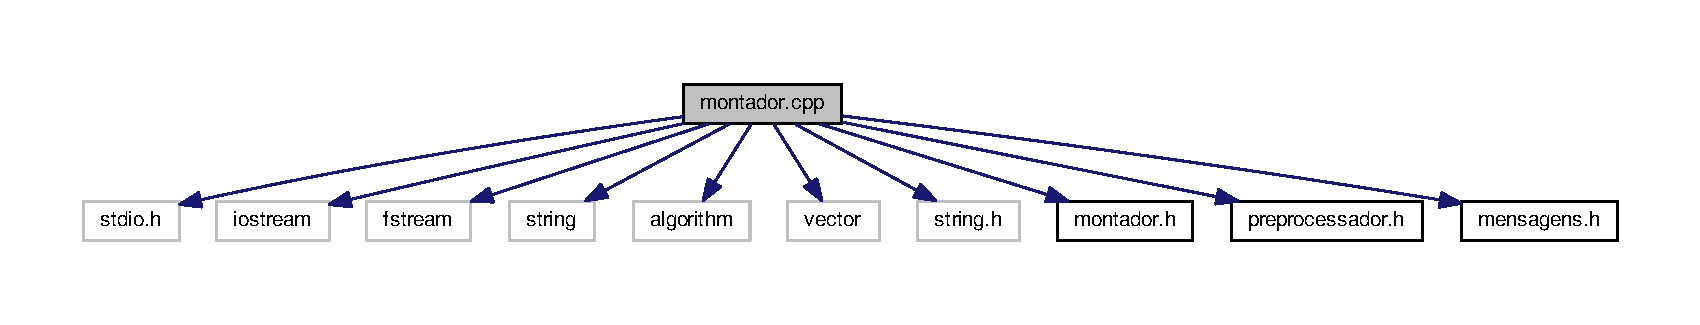
\includegraphics[width=350pt]{montador_8cpp__incl}
\end{center}
\end{figure}
\subsection*{Funções}
\begin{DoxyCompactItemize}
\item 
int \hyperlink{montador_8cpp_a43bfc12a769340a4db437ddb8d4adc03}{montador} (int argc, char $\ast$argv\mbox{[}$\,$\mbox{]})
\end{DoxyCompactItemize}


\subsection{Documentação das funções}
\hypertarget{montador_8cpp_a43bfc12a769340a4db437ddb8d4adc03}{\index{montador.\-cpp@{montador.\-cpp}!montador@{montador}}
\index{montador@{montador}!montador.cpp@{montador.\-cpp}}
\subsubsection[{montador}]{\setlength{\rightskip}{0pt plus 5cm}int montador (
\begin{DoxyParamCaption}
\item[{int}]{argc, }
\item[{char $\ast$}]{argv\mbox{[}$\,$\mbox{]}}
\end{DoxyParamCaption}
)}}\label{montador_8cpp_a43bfc12a769340a4db437ddb8d4adc03}
Montador

\begin{DoxyAuthor}{Autor}
Rafael e João Pedro Franch 
\end{DoxyAuthor}


Definido na linha 21 do ficheiro montador.\-cpp.



Este é o diagrama das funções que utilizam esta função\-:
\nopagebreak
\begin{figure}[H]
\begin{center}
\leavevmode
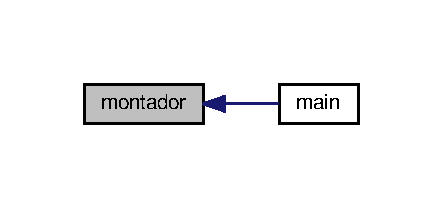
\includegraphics[width=212pt]{montador_8cpp_a43bfc12a769340a4db437ddb8d4adc03_icgraph}
\end{center}
\end{figure}



\hypertarget{montador_8h}{\section{Referência ao ficheiro montador.\-h}
\label{montador_8h}\index{montador.\-h@{montador.\-h}}
}
Este grafo mostra quais são os ficheiros que incluem directamente ou indirectamente este ficheiro\-:
\nopagebreak
\begin{figure}[H]
\begin{center}
\leavevmode
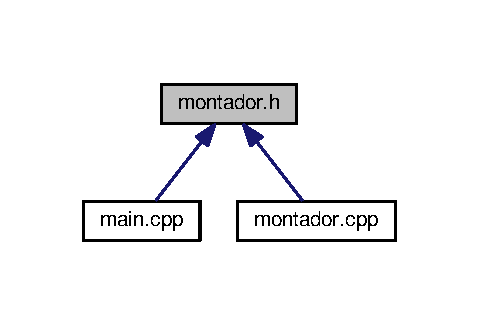
\includegraphics[width=230pt]{montador_8h__dep__incl}
\end{center}
\end{figure}
\subsection*{Funções}
\begin{DoxyCompactItemize}
\item 
int \hyperlink{montador_8h_a43bfc12a769340a4db437ddb8d4adc03}{montador} (int argc, char $\ast$argv\mbox{[}$\,$\mbox{]})
\end{DoxyCompactItemize}


\subsection{Documentação das funções}
\hypertarget{montador_8h_a43bfc12a769340a4db437ddb8d4adc03}{\index{montador.\-h@{montador.\-h}!montador@{montador}}
\index{montador@{montador}!montador.h@{montador.\-h}}
\subsubsection[{montador}]{\setlength{\rightskip}{0pt plus 5cm}int montador (
\begin{DoxyParamCaption}
\item[{int}]{argc, }
\item[{char $\ast$}]{argv\mbox{[}$\,$\mbox{]}}
\end{DoxyParamCaption}
)}}\label{montador_8h_a43bfc12a769340a4db437ddb8d4adc03}
Montador

\begin{DoxyAuthor}{Autor}
Rafael e João Pedro Franch 
\end{DoxyAuthor}


Definido na linha 21 do ficheiro montador.\-cpp.



Este é o diagrama das funções que utilizam esta função\-:
\nopagebreak
\begin{figure}[H]
\begin{center}
\leavevmode
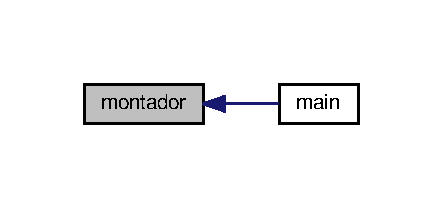
\includegraphics[width=212pt]{montador_8h_a43bfc12a769340a4db437ddb8d4adc03_icgraph}
\end{center}
\end{figure}



\hypertarget{preprocessador_8cpp}{\section{Referência ao ficheiro preprocessador.\-cpp}
\label{preprocessador_8cpp}\index{preprocessador.\-cpp@{preprocessador.\-cpp}}
}
{\ttfamily \#include $<$sstream$>$}\\*
{\ttfamily \#include \char`\"{}mensagens.\-h\char`\"{}}\\*
{\ttfamily \#include \char`\"{}preprocessador.\-h\char`\"{}}\\*
Diagrama de dependências de inclusão para preprocessador.\-cpp\-:
\nopagebreak
\begin{figure}[H]
\begin{center}
\leavevmode
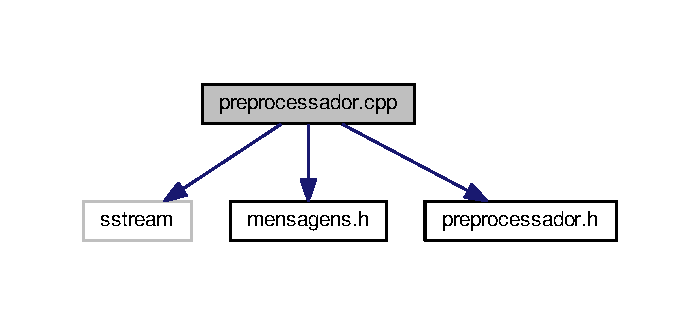
\includegraphics[width=336pt]{preprocessador_8cpp__incl}
\end{center}
\end{figure}
\subsection*{Funções}
\begin{DoxyCompactItemize}
\item 
int \hyperlink{preprocessador_8cpp_a9e48831dcb56bc3edbcad2a43c6d1c44}{pre\-Processador} (int argc, char $\ast$$\ast$argv)
\end{DoxyCompactItemize}


\subsection{Documentação das funções}
\hypertarget{preprocessador_8cpp_a9e48831dcb56bc3edbcad2a43c6d1c44}{\index{preprocessador.\-cpp@{preprocessador.\-cpp}!pre\-Processador@{pre\-Processador}}
\index{pre\-Processador@{pre\-Processador}!preprocessador.cpp@{preprocessador.\-cpp}}
\subsubsection[{pre\-Processador}]{\setlength{\rightskip}{0pt plus 5cm}int pre\-Processador (
\begin{DoxyParamCaption}
\item[{int}]{argc, }
\item[{char $\ast$$\ast$}]{argv}
\end{DoxyParamCaption}
)}}\label{preprocessador_8cpp_a9e48831dcb56bc3edbcad2a43c6d1c44}


Definido na linha 12 do ficheiro preprocessador.\-cpp.



Este é o diagrama das funções que utilizam esta função\-:
\nopagebreak
\begin{figure}[H]
\begin{center}
\leavevmode
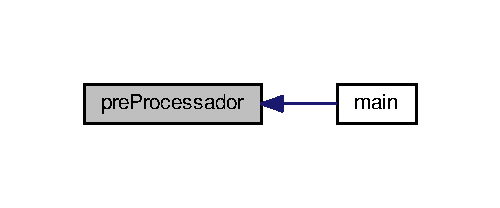
\includegraphics[width=240pt]{preprocessador_8cpp_a9e48831dcb56bc3edbcad2a43c6d1c44_icgraph}
\end{center}
\end{figure}



\hypertarget{preprocessador_8h}{\section{Referência ao ficheiro preprocessador.\-h}
\label{preprocessador_8h}\index{preprocessador.\-h@{preprocessador.\-h}}
}
Este grafo mostra quais são os ficheiros que incluem directamente ou indirectamente este ficheiro\-:
\nopagebreak
\begin{figure}[H]
\begin{center}
\leavevmode
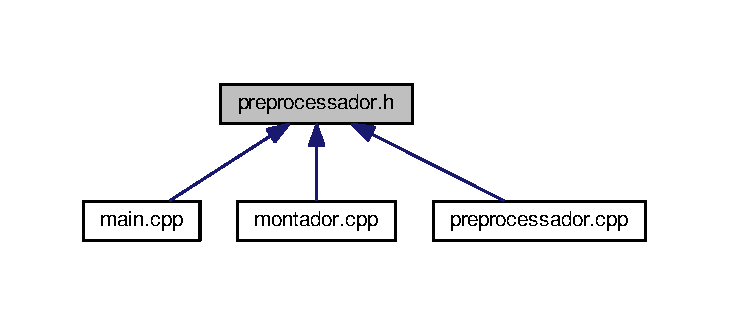
\includegraphics[width=350pt]{preprocessador_8h__dep__incl}
\end{center}
\end{figure}
\subsection*{Funções}
\begin{DoxyCompactItemize}
\item 
int \hyperlink{preprocessador_8h_a9e48831dcb56bc3edbcad2a43c6d1c44}{pre\-Processador} (int argc, char $\ast$$\ast$argv)
\end{DoxyCompactItemize}


\subsection{Documentação das funções}
\hypertarget{preprocessador_8h_a9e48831dcb56bc3edbcad2a43c6d1c44}{\index{preprocessador.\-h@{preprocessador.\-h}!pre\-Processador@{pre\-Processador}}
\index{pre\-Processador@{pre\-Processador}!preprocessador.h@{preprocessador.\-h}}
\subsubsection[{pre\-Processador}]{\setlength{\rightskip}{0pt plus 5cm}int pre\-Processador (
\begin{DoxyParamCaption}
\item[{int}]{argc, }
\item[{char $\ast$$\ast$}]{argv}
\end{DoxyParamCaption}
)}}\label{preprocessador_8h_a9e48831dcb56bc3edbcad2a43c6d1c44}


Definido na linha 16 do ficheiro preprocessador.\-cpp.



Este é o diagrama das funções que utilizam esta função\-:
\nopagebreak
\begin{figure}[H]
\begin{center}
\leavevmode
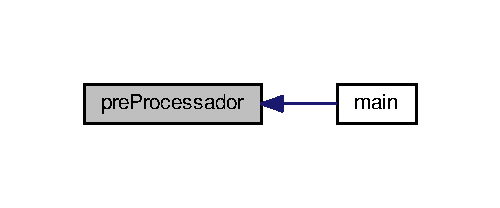
\includegraphics[width=240pt]{preprocessador_8h_a9e48831dcb56bc3edbcad2a43c6d1c44_icgraph}
\end{center}
\end{figure}



%--- End generated contents ---

% Index
\newpage
\phantomsection
\addcontentsline{toc}{chapter}{Índice}
\printindex

\end{document}
